\chapter{Composite Bosons, Spin, and the Dirac Equation}

This lecture begins in response to a question, not in the style of an announced theorem. We are first asked to face a tension left over from earlier meetings: if a hydrogen atom is a boson built from fermions, how can two such atoms occupy the same state without violating the Pauli principle? From there the lecture makes an explicit pivot to spin, because the same mathematics will later return as isospin, color, and internal symmetry more generally. Finally we come back to the Dirac equation, where the same two-by-two structure appears twice: once as spin and once as the doubling into positive- and negative-energy solutions. These notes follow Leonard Susskind's Lecture 8, with curation by LazyingArt LLC, and try to keep the sense that the argument is being unfolded at the board.

\section{Exchange Symmetry and Composite Bosons}

Let us begin exactly where the lecture begins. If two identical bosons are described by a wavefunction \(\psi(x,y)\), then \(x\) and \(y\) are not names for two different species. They are only the two particle slots. The rule is

\begin{equation}
\psi_B(x,y)=\psi_B(y,x),
\qquad
\psi_F(x,y)=-\psi_F(y,x),
\end{equation}

for bosons and fermions respectively. This is the mathematical expression of indistinguishability: exchanging the labels does nothing for bosons and changes the sign for fermions.

From this alone we can already answer one part of the opening question. Two bosons can certainly be in the same one-particle state. If \(\varphi(x)\) is a one-particle wavefunction, then

\begin{equation}
\psi(x,y)=\varphi(x)\varphi(y)
\end{equation}

is a perfectly good two-boson wavefunction. The reason is simple and the lecture insists on it: wavefunctions are not operators. They are ordinary complex-valued functions, so

\begin{equation}
\varphi(x)\varphi(y)=\varphi(y)\varphi(x).
\end{equation}

Thus the product state is automatically symmetric. For fermions the same construction fails, since

\begin{equation}
\varphi(x)\varphi(y)\neq -\,\varphi(y)\varphi(x)
\end{equation}

unless the state is identically zero. This is the elementary form of the exclusion principle.

The next move in the lecture is constructive. Suppose we start with a two-particle wavefunction \(\phi(x,y)\) which is neither symmetric nor antisymmetric. Then we may manufacture from it the two combinations

\begin{align}
\psi_{\mathrm{sym}}(x,y) &= \phi(x,y)+\phi(y,x),\\
\psi_{\mathrm{asym}}(x,y) &= \phi(x,y)-\phi(y,x).
\end{align}

Up to normalization, these are the bosonic and fermionic projections of the original state. The point is not merely that such states exist. The point is that this add-or-subtract rule is exactly the tool we will need once the lecture raises the stakes from two particles to two hydrogen atoms.

\section{Two Hydrogen Atoms as a Four-Fermion System}

Now we move from the toy two-body discussion to the actual physical question. A hydrogen atom is made of an electron and a proton, and both are fermions. So two hydrogen atoms form a four-body system with two identical electrons and two identical protons.

Let us label the electron coordinates by \(x_1,x_2\) and the proton coordinates by \(y_1,y_2\). The four-body wavefunction must satisfy

\begin{equation}
\Psi(x_1,x_2;y_1,y_2)=-\Psi(x_2,x_1;y_1,y_2),
\end{equation}

because the electrons are identical fermions, and also

\begin{equation}
\Psi(x_1,x_2;y_1,y_2)=-\Psi(x_1,x_2;y_2,y_1),
\end{equation}

because the protons are identical fermions. These are the only rules we need at this stage.

The lecture constructs the state in two steps. We start with the naive product of two one-atom wavefunctions,
\[
\psi(x_1,y_1)\phi(x_2,y_2),
\]
where \(\psi\) describes one hydrogen atom and \(\phi\) the other. In general this is not yet acceptable, because it is not antisymmetric in the electron labels and not antisymmetric in the proton labels.

So first we antisymmetrize in the electron coordinates:

\begin{equation}
\Psi_x(x_1,x_2;y_1,y_2)
=
\psi(x_1,y_1)\phi(x_2,y_2)
-
\psi(x_2,y_1)\phi(x_1,y_2).
\end{equation}

This state now changes sign under \(x_1\leftrightarrow x_2\), but it still does not have the right behavior under \(y_1\leftrightarrow y_2\). So we do exactly the same thing once more, now with the proton coordinates, and obtain

\begin{align}
\Psi_{2H}(x_1,x_2;y_1,y_2)
&=
\Psi_x(x_1,x_2;y_1,y_2)-\Psi_x(x_1,x_2;y_2,y_1)\\
&=
\psi(x_1,y_1)\phi(x_2,y_2)
-\psi(x_2,y_1)\phi(x_1,y_2)\nonumber\\
&\quad
-\psi(x_1,y_2)\phi(x_2,y_1)
+\psi(x_2,y_2)\phi(x_1,y_1).
\end{align}

This four-term expression is a cautious reconstruction of the oral derivation. In the transcript the delivery is compressed and partly garbled, but the sign pattern \(+,-,-,+\) is fixed by the two successive antisymmetrizations and is the part that matters.

Now we come to the local payoff. What happens if we interchange the two whole atoms? That is not just \(x_1\leftrightarrow x_2\), and not just \(y_1\leftrightarrow y_2\), but both at once:

\[
(x_1,y_1)\longleftrightarrow(x_2,y_2).
\]

Under the electron exchange we get one minus sign. Under the proton exchange we get another. Therefore

\begin{equation}
\Psi_{2H}(x_2,x_1;y_2,y_1)=\Psi_{2H}(x_1,x_2;y_1,y_2).
\end{equation}

Minus times minus is plus. So the two-atom state is symmetric under interchange of atom \(1\) and atom \(2\). This is the precise sense in which the hydrogen atoms behave as bosons.

The lecture is careful here not to let this symmetry statement drift into a statement about energetics. The exchange rule is one thing; whether two atoms can literally be pushed on top of each other in space is another. Strong repulsive effects may make that energetically impossible. But that does not change the symmetry classification. Two bosonic atoms can occupy the same momentum state even if putting them at the same point in space is costly.

\subsection{Question \& Answer}

\paragraph{Question.} How can two bosonic atoms be in the same state if their constituent fermions cannot?

\paragraph{Answer.} This is where the lecture deliberately slows down. Let us now set the two one-atom wavefunctions equal, \(\phi=\psi\). Then the two-atom state becomes

\begin{align}
\Psi_{\mathrm{same}}(x_1,x_2;y_1,y_2)
&=
\psi(x_1,y_1)\psi(x_2,y_2)
-\psi(x_2,y_1)\psi(x_1,y_2)\nonumber\\
&\quad
-\psi(x_1,y_2)\psi(x_2,y_1)
+\psi(x_2,y_2)\psi(x_1,y_1)\\
&=
2\Big[\psi(x_1,y_1)\psi(x_2,y_2)-\psi(x_2,y_1)\psi(x_1,y_2)\Big].
\end{align}

This is not zero in general. So two atoms can indeed occupy the same atomic state.

But now let us test the constituent fermions directly. If we force the two electrons to be at the same point, we set \(x_1=x_2=x\). Then

\begin{align}
\Psi_{\mathrm{same}}(x,x;y_1,y_2)
&=
2\Big[\psi(x,y_1)\psi(x,y_2)-\psi(x,y_1)\psi(x,y_2)\Big]\\
&=0.
\end{align}

Likewise, if we set \(y_1=y_2\), the proton sector vanishes. So the apparent paradox is resolved in exactly the way the lecture wants us to see it: the atoms may occupy the same atomic state, but the antisymmetrization has already projected out the pieces in which the identical constituent fermions occupy the same constituent state.

This is also why the lecture keeps separating ``same state'' from ``same place.'' A momentum eigenstate is spread out in space. Two bosonic atoms may live in the same momentum state without their two electrons ever being in the same place. The Pauli principle is still fully at work inside the four-body wavefunction.

\section{Half-Spin as a Two-State Quantum System}

At this point the lecture makes an explicit reset: let us come back to spin. The reason for lingering here is not only that electrons have spin, but that the mathematics of spin is the mathematics we will later reuse for isospin, color, and internal symmetry more broadly.

We begin in the rest-frame, non-relativistic spirit of the lecture. Forget the position of the electron for the moment. Forget its momentum. Think of the electron as nailed to the wall, so that the only thing we are asking about is its spin. In that reduced problem the state space is two-dimensional.

With \(\hbar=1\), the spin operators obey the standard commutation relations

\begin{equation}
[S_x,S_y]=iS_z,\qquad [S_y,S_z]=iS_x,\qquad [S_z,S_x]=iS_y,
\end{equation}

together with the raising and lowering operators

\begin{equation}
S_\pm = S_x \pm iS_y.
\end{equation}

For a spin-\(\tfrac12\) particle, \(S_z\) takes the values \(+\tfrac12\) and \(-\tfrac12\). So every spin state may be written as a two-component column,

\begin{equation}
\psi=
\begin{pmatrix}
\alpha\\
\beta
\end{pmatrix},
\qquad
|\alpha|^2=P(\text{up along }z),
\qquad
|\beta|^2=P(\text{down along }z).
\end{equation}

This is spin space, not ordinary space. Operators on this space become \(2\times2\) matrices. Choosing \(S_z\) to be diagonal, we may write

\begin{equation}
S_i=\frac12 \sigma_i,
\end{equation}

with the Pauli matrices

\begin{equation}
\sigma_x=
\begin{pmatrix}
0&1\\
1&0
\end{pmatrix},
\qquad
\sigma_y=
\begin{pmatrix}
0&-i\\
i&0
\end{pmatrix},
\qquad
\sigma_z=
\begin{pmatrix}
1&0\\
0&-1
\end{pmatrix}.
\end{equation}

The lecture then proceeds in the most concrete way possible: we solve the eigenvalue problems one axis at a time. Since \(S_i=\tfrac12 \sigma_i\), it is convenient to solve the eigenvalue equations for \(\sigma_i\), whose eigenvalues are \(\pm1\), and divide by \(2\) at the end if we want the eigenvalues of \(S_i\).

For \(\sigma_z\), we solve

\begin{align}
\sigma_z
\begin{pmatrix}
\alpha\\
\beta
\end{pmatrix}
&=
+
\begin{pmatrix}
\alpha\\
\beta
\end{pmatrix},
&
\sigma_z
\begin{pmatrix}
\alpha\\
\beta
\end{pmatrix}
&=
-
\begin{pmatrix}
\alpha\\
\beta
\end{pmatrix}.
\end{align}

The first equation gives \(\beta=0\), the second gives \(\alpha=0\). Thus the normalized eigenvectors are

\begin{equation}
|+\!z\rangle=
\begin{pmatrix}
1\\
0
\end{pmatrix},
\qquad
|-\!z\rangle=
\begin{pmatrix}
0\\
1
\end{pmatrix}.
\end{equation}

\begin{figure}[t]
\centering

\includegraphics[width=0.74\textwidth]{lecture_08_figure_02.png}
\caption{Pauli-\(\sigma_z\) eigenvalue equation.}
\end{figure}

The lecture then changes experiment: instead of measuring the \(z\)-component, measure the \(x\)-component. In that case

\begin{equation}
\sigma_x
\begin{pmatrix}
\alpha\\
\beta
\end{pmatrix}
=
\begin{pmatrix}
\beta\\
\alpha
\end{pmatrix}.
\end{equation}

So the \(+1\) eigenvalue problem says \(\alpha=\beta\), while the \(-1\) eigenvalue problem says \(\beta=-\alpha\). After normalization we find

\begin{equation}
|+\!x\rangle=\frac{1}{\sqrt2}
\begin{pmatrix}
1\\
1
\end{pmatrix},
\qquad
|-\!x\rangle=\frac{1}{\sqrt2}
\begin{pmatrix}
1\\
-1
\end{pmatrix}.
\end{equation}

This is precisely the point the lecture wants to emphasize: a state definite along the \(x\)-axis is a linear combination of the \(z\)-up and \(z\)-down states.

\begin{figure}[t]
\centering

\includegraphics[width=0.74\textwidth]{lecture_08_figure_03.png}
\caption{\(\sigma_x\) eigenvector condition.}
\end{figure}

For \(\sigma_y\) the lecture moves faster, and here the live board work visibly hesitates over the sign assignment. The safe statement is the standard one:

\begin{equation}
|+\!y\rangle=\frac{1}{\sqrt2}
\begin{pmatrix}
1\\
i
\end{pmatrix},
\qquad
|-\!y\rangle=\frac{1}{\sqrt2}
\begin{pmatrix}
1\\
-i
\end{pmatrix},
\end{equation}

up to an overall phase. The new ingredient is the relative factor of \(i\). That is why an electron polarized along the \(y\)-axis is not the same state as one polarized along the \(x\)-axis, even though both give equal probabilities for \(z\)-up and \(z\)-down.

\begin{figure}[t]
\centering

\includegraphics[width=0.82\textwidth]{lecture_08_figure_04.png}
\caption{\(\sigma_y\) eigenvectors and spin-matrix summary.}
\end{figure}

So the spin-\(\tfrac12\) story is now in place. We have a two-state system, a two-component spinor, and three matrices that tell us how to ask for spin along the \(x\), \(y\), and \(z\) directions. The lecture lingers here because exactly this formal structure will be used again in other guises later on.

\section{Spin-1 and the Meaning of Multi-Component Wavefunctions}

The lecture next asks us to do the same thing for spin \(1\). Now the \(z\)-component can take the values \(+1\), \(0\), and \(-1\), so the state space is three-dimensional. Again there are many equivalent matrix realizations, and Susskind chooses one which is deliberately symmetric among \(x\), \(y\), and \(z\), rather than one with \(S_z\) diagonal from the start.

A convenient reconstruction matching the spoken pattern is

\begin{equation}
S_x
=
i
\begin{pmatrix}
0&0&0\\
0&0&1\\
0&-1&0
\end{pmatrix},
\qquad
S_y
=
i
\begin{pmatrix}
0&0&-1\\
0&0&0\\
1&0&0
\end{pmatrix},
\qquad
S_z
=
i
\begin{pmatrix}
0&1&0\\
-1&0&0\\
0&0&0
\end{pmatrix}.
\end{equation}

These are purely imaginary and antisymmetric, and each one has the same pattern: a \(1\), a \(-1\), and a vanishing row and column corresponding to its letter. In this basis \(S_z\) is not diagonal, so we find the states of definite \(m_s\) by solving the eigenvalue problem directly. The resulting eigenvectors are

\begin{equation}
|m_s=+1\rangle
=
\frac{1}{\sqrt2}
\begin{pmatrix}
1\\
-i\\
0
\end{pmatrix},
\qquad
|m_s=-1\rangle
=
\frac{1}{\sqrt2}
\begin{pmatrix}
1\\
i\\
0
\end{pmatrix},
\qquad
|m_s=0\rangle
=
\begin{pmatrix}
0\\
0\\
1
\end{pmatrix}.
\end{equation}

These are not written in the most familiar textbook basis, but that is exactly the point of the lecture here: the representation is not unique. What matters is the algebra and the resulting eigenvectors.

The lecture then makes another important transition. Up to this point we have been discussing finite-dimensional spin spaces by themselves. Now let us return to a real particle moving in ordinary space. Position and spin may be measured simultaneously, whereas different spin components do not commute with one another. So the wavefunction of a moving spin-\(\tfrac12\) particle becomes a position-dependent two-component object,

\begin{equation}
\psi(x)=
\begin{pmatrix}
\psi_\uparrow(x)\\
\psi_\downarrow(x)
\end{pmatrix},
\end{equation}

with

\begin{equation}
|\psi_\uparrow(x)|^2=P(\uparrow \text{ at }x),
\qquad
|\psi_\downarrow(x)|^2=P(\downarrow \text{ at }x).
\end{equation}

For a spin-1 particle the same structure reappears with three components,

\begin{equation}
\phi(x)=
\begin{pmatrix}
\phi_1(x)\\
\phi_2(x)\\
\phi_3(x)
\end{pmatrix}.
\end{equation}

At each point in space we now have a vector in spin space. This is one of the characteristic moves in the lecture: we take the finite-dimensional story and reproduce it point by point in space.

\subsection{Question \& Answer}

\paragraph{Question.} Is \(\psi_1\) itself a probability?

\paragraph{Answer.} No. A component of the column is an amplitude in some chosen basis. The probability for a physical spin outcome is obtained only after projection onto the appropriate eigenvector.

If \(|m_s\rangle\) is the normalized eigenvector for the spin outcome \(m_s\), then the rule is

\begin{equation}
P(m_s\mid x)=|\langle m_s|\phi(x)\rangle|^2.
\end{equation}

This is the principle the lecture wants to stabilize, and it is more important than the live arithmetic, which Susskind himself recognizes is shaky at the board.

For the spin-1 basis above, we obtain

\begin{align}
P(+1\mid x)
&=
\left|
\frac{1}{\sqrt2}
\begin{pmatrix}
1&i&0
\end{pmatrix}
\begin{pmatrix}
\phi_1(x)\\
\phi_2(x)\\
\phi_3(x)
\end{pmatrix}
\right|^2
=
\frac12\left|\phi_1(x)+i\phi_2(x)\right|^2,\\
P(-1\mid x)
&=
\frac12\left|\phi_1(x)-i\phi_2(x)\right|^2,\\
P(0\mid x)
&=
\left|
\begin{pmatrix}
0&0&1
\end{pmatrix}
\begin{pmatrix}
\phi_1(x)\\
\phi_2(x)\\
\phi_3(x)
\end{pmatrix}
\right|^2
=
|\phi_3(x)|^2.
\end{align}

The lecture's temporary mistake in this segment comes from informally treating \(\phi_1\) and \(\phi_2\) as real. Once we keep them complex, the projection rule gives the correct answer immediately. That is the point worth carrying forward.

\section{Dirac Matrices in Block Form}

Now let us come back to the Dirac equation. In the lecture it is written as

\begin{equation}
i\partial_t\Psi
=
-\,i\,\alpha_i\,\partial_i\Psi
+
m\beta\Psi,
\qquad i=1,2,3,
\end{equation}

where \(\Psi\) is a four-component spinor and repeated spatial indices are summed.

If we test the equation on a plane wave, the right-hand side becomes an algebraic operator of the form

\begin{equation}
\omega \Psi = \left(\alpha_i k_i + m\beta\right)\Psi.
\end{equation}

The lecture then reminds us why the \(\alpha_i\) and \(\beta\) cannot be arbitrary. Once we square this operator, we must recover the relativistic dispersion relation

\begin{equation}
\omega^2 = k^2 + m^2.
\end{equation}

That means, first, that the square terms must behave properly:

\begin{equation}
\alpha_i^2=1,
\qquad
\beta^2=1.
\end{equation}

Second, all the mixed terms must disappear. So for \(i\neq j\),

\begin{equation}
\alpha_i\alpha_j+\alpha_j\alpha_i=0,
\qquad
\alpha_i\beta+\beta\alpha_i=0.
\end{equation}

All this is summarized compactly as

\begin{equation}
\{\alpha_i,\alpha_j\}=2\delta_{ij},
\qquad
\{\alpha_i,\beta\}=0,
\qquad
\beta^2=1.
\end{equation}

Without \(\beta\), the Pauli matrices would already solve the problem in \(2\times2\) form. But with the extra matrix \(\beta\), three \(2\times2\) matrices are no longer enough. That is why the minimal representation is \(4\times4\). This is one of the lecture's important motivational beats: the four-component Dirac spinor is not put in by hand as decoration. It is forced on us by the algebra.

The lecture then chooses a \(2\times2\) block representation. For the \(\alpha_i\) one convenient form is

\begin{equation}
\alpha_i=
\begin{pmatrix}
\sigma_i&0\\
0&-\sigma_i
\end{pmatrix}.
\end{equation}

For \(\beta\), the transcript compares this representation with an earlier equivalent one, so the chalk marks are noisy. The form consistent with the rest-frame discussion a few minutes later is

\begin{equation}
\beta=
\begin{pmatrix}
0&I\\
I&0
\end{pmatrix},
\qquad
I=
\begin{pmatrix}
1&0\\
0&1
\end{pmatrix}.
\end{equation}

\begin{figure}[t]
\centering

\includegraphics[width=0.68\textwidth]{lecture_08_figure_05.png}
\caption{Block form of \(\alpha_i\) from Pauli matrices.}
\end{figure}

\begin{figure}[t]
\centering
\begin{tikzpicture}[scale=1.0]
\draw (0,0) rectangle (4,4);
\draw (2,0)--(2,4);
\draw (0,2)--(4,2);
\node at (1,3) {$\sigma_i$};
\node at (3,3) {$0$};
\node at (1,1) {$0$};
\node at (3,1) {$-\sigma_i$};
\end{tikzpicture}
\caption{A clean block-matrix version of the board organization for \(\alpha_i\).}
\end{figure}

This is where the lecture explicitly introduces the theme of two distinct two-by-two structures. One two-by-two-ness is the block decomposition itself. The other is the Pauli-matrix structure inside each block. The physical meaning of that double doubling is what the rest-frame analysis is about to reveal.

\section{The Rest-Frame Dirac Equation, Energy Doubling, and Positrons}

Susskind now asks for the easiest possible place to see what the four components mean. The easiest place is \(k=0\), the particle at rest. If the momentum vanishes, the wavefunction has no spatial dependence, the \(\alpha_i\partial_i\) terms drop out, and the Dirac equation becomes purely a time-evolution equation.

The chalkboard at this moment still carries an extra factor of \(i\), but the lecture immediately corrects it in the subsequent algebra. The cleaned equation is

\begin{equation}
i\,\partial_t\Psi = m\,\beta\,\Psi.
\end{equation}

\begin{figure}[t]
\centering

\includegraphics[width=0.76\textwidth]{lecture_08_figure_06.png}
\caption{Rest-frame Dirac equation.}
\end{figure}

Now divide the four-component Dirac spinor into two two-component pieces:

\begin{equation}
\Psi=
\begin{pmatrix}
\psi_+\\
\psi_-
\end{pmatrix}.
\end{equation}

In this notation \(\beta\) simply swaps the upper and lower blocks. So the rest-frame Dirac equation says

\begin{equation}
i\dot{\psi}_+=m\psi_-,
\qquad
i\dot{\psi}_-=m\psi_+.
\end{equation}

This is the whole upshot of the rest-frame Dirac equation. The lecture then asks how to simplify it further. The answer is: add and subtract. Define

\begin{equation}
\chi_+ = \psi_+ + \psi_-,
\qquad
\chi_- = \psi_+ - \psi_-.
\end{equation}

Then the two combinations decouple:

\begin{align}
i\partial_t\chi_+ &= m\chi_+,\\
i\partial_t\chi_- &= -m\chi_-.
\end{align}

So a state of definite frequency has either

\begin{equation}
\omega=+m
\qquad \text{or} \qquad
\omega=-m.
\end{equation}

That is the first two-by-two-ness: positive- and negative-energy solutions.

Moreover, in the positive-energy branch we have \(\psi_-=\psi_+\), while in the negative-energy branch we have \(\psi_-=-\psi_+\). So we may write the rest-frame solutions as

\begin{equation}
\Psi_{\mathrm{pos}}=
\begin{pmatrix}
\chi\\
\chi
\end{pmatrix},
\qquad
\Psi_{\mathrm{neg}}=
\begin{pmatrix}
\chi\\
-\chi
\end{pmatrix},
\end{equation}

with \(\chi\) an arbitrary two-component spinor. This is the second two-by-two-ness: the two entries of \(\chi\) are just the familiar spin-\(\tfrac12\) doublet.

\begin{figure}[t]
\centering
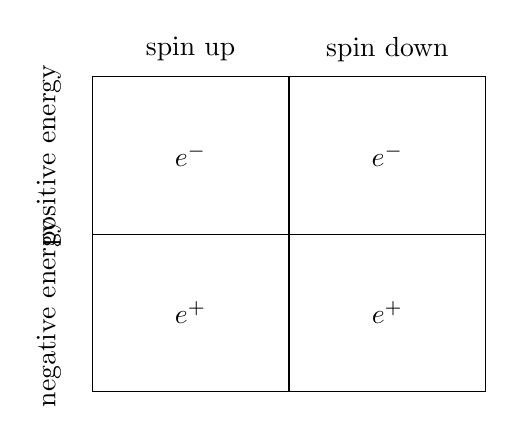
\begin{tikzpicture}[scale=1.0]
\draw (0,0) rectangle (5,4);
\draw (2.5,0)--(2.5,4);
\draw (0,2)--(5,2);
\node at (1.25,4.35) {spin up};
\node at (3.75,4.35) {spin down};
\node[rotate=90] at (-0.55,3) {positive energy};
\node[rotate=90] at (-0.55,1) {negative energy};
\node at (1.25,3) {$e^-$};
\node at (3.75,3) {$e^-$};
\node at (1.25,1) {$e^+$};
\node at (3.75,1) {$e^+$};
\end{tikzpicture}
\caption{The two independent doublings in the Dirac spinor: energy sign and spin sign.}
\end{figure}

This is exactly the interpretation the lecture wants us to keep. One doubling is positive versus negative energy. The other doubling is spin up versus spin down. The four components of the Dirac spinor are not four spacetime coordinates. They are the smallest representation of this algebraic structure.

\subsection{Question \& Answer}

\paragraph{Question.} What is the physical meaning of the negative-energy solutions?

\paragraph{Answer.} The lecture answers this in the Dirac-sea language. Negative frequency means negative energy. If negative-energy electron states exist, then the vacuum is not the state in which they are empty. The vacuum is the state in which they are all filled. Because electrons are fermions, no more than one electron may occupy a given negative-energy state.

Now take one of those negative-energy electrons and move it into a positive-energy state. What remains? A positive-energy electron together with the absence of a negative-energy electron. That absence is the hole in the Dirac sea, and it behaves as a positive-energy particle of opposite charge: a positron.

This is why the lecture says that one doubling becomes electrons and positrons, while the other doubling becomes spin. The Dirac equation predicts not only spin-\(\tfrac12\) particles, but spin-\(\tfrac12\) particles that come in particle-antiparticle pairs.

The lecture then follows the next question rather than shutting it down. Why do higher negative-energy electrons not fall into the hole? The answer is that they can. When that happens, we can interpret the process as the positron changing its state. A change of state of this kind may emit photons. Likewise, when a positive-energy electron and a positron disappear, we call that positron-electron annihilation, and photons carry away the conserved energy and momentum.

The final clarification is important. One must not imagine an unrestricted downward cascade in which everything simply falls forever. Energy conservation by itself is not enough; momentum conservation matters as well. The lecture closes by pointing out that this is no stranger than the fact that a free electron in empty space cannot simply continue radiating photons and sliding to lower and lower energy. The same conservation laws constrain the positron picture.

There is also one last mathematical moral. In the rest frame the \(\alpha_i\) do not appear in the time-evolution equation, so spin is not displayed dynamically there in the same simple way that energy doubling is. But after the positive- and negative-energy pieces have been separated, the remaining two-component structure is still present. That residual two-component freedom is the spin.

\section{Summary}

The lecture ties together three threads and lets each one illuminate the next. First, a composite boson can be built from fermions because the two constituent minus signs under atom exchange multiply to a plus sign. Second, spin is the quantum mechanics of finite-dimensional state spaces, and its algebra is worth learning because the same structure will reappear in later parts of particle physics. Third, the Dirac equation contains two independent doublings: one is the familiar spin-\(\tfrac12\) doubling, and the other is the split into positive- and negative-energy branches. In the lecture's own rhythm, two minus signs become a boson, one relative phase \(i\) distinguishes \(y\) from \(x\), and one four-by-four matrix structure becomes electrons, positrons, and spin.